\documentclass{beamer}
\usepackage[utf8]{inputenc}
\usepackage[spanish, mexico]{babel}
\usepackage{amsmath}
\usepackage{amsfonts}
\usepackage{amssymb}
% url
\usepackage{hyperref}
% Configuración de la presentación
\usetheme{Ilmenau} % Tema por defecto
\usecolortheme{default} % Colores por defecto
% íconos
\usepackage{fontawesome5}

% colores
\usepackage{xcolor} % definir colores
\usepackage{tcolorbox} % cajas de color
\definecolor{CODE}{RGB}{229, 232, 232}
% comandos
\newcommand{\codigo}[1]{\colorbox{CODE}{\texttt{#1}}}

% Diapositiva de introducción
\title{Business Intelligence con Shiny}
%\subtitle{Planteamiento del Problema}
\author{Act. Edgar Ruiz Tovar}
\institute{Actuarios por México}
\date{12 de marzo de 2024}

% Contenido de la presentación
\begin{document}
    % Diapositiva de título
    \begin{frame}
      \titlepage
    \end{frame}
    % Primer diapositiva: Planteamiento del problema
    % slide 1
\begin{frame}
    \frametitle{Planteamiento del problema}
    \begin{itemize}
        \item<1-> Imagina que empiezas a trabajar en la Aseguradora \textit{XXX, S.A. de C.V.}
        \item<2-> Esta aseguradora tiene permiso para operar \textbf{múltiples ramos}. 
        \item<3-> En tu primer semana conoces a tu equipo de trabajo, el cual es un equipo \underline{integral} pues tiene diferentes perfiles profesionales.
        \item<4-> Ellos saben que por estudiar Actuaría...
        \item<5-> Eres bueno con los números.
        \item<6-> A la siguiente semana vas con tu jefe y te pide que realices un \textit{estudio de mercado} porque quiere presentarle al Director unas cifras para saber si le conviene o no, crear cierto producto.
  \end{itemize}
\end{frame}
    % Segunda diapositiva: Estudio de Mercado
    % slide 2
\begin{frame}
    \frametitle{Estudio de mercado}
    \begin{itemize}
        \item<1-> ¿Cuánto se emitió en la cuenta \textit{xxx} del trimestre \textit{ttt}?. En particular enfócate en los ramos operados \textit{aaa}, \textit{bbb} y \textit{ccc}.
        \item<2-> ¿Cuál fue el monto de la cuenta \textit{xxx} por el ramo operado \textit{aaa}?, ¿y el año pasado?
        \item<3-> ¿Qué empresa es líder en el mercado asegurador en el ramo \textit{aaa}?, ¿dónde nos encontramos?
        \item<4-> ¿Seguimos la tendendencia del sector asegurador en la emisión de \textit{aaa}?
        \item<5-> ¿Cómo nos podemos comparar respecto a nuestra competencia?
        \item<6-> ¿Hemos tenido crecimientos en los ramos operados \textit{aaa} y \textit{bbb} respecto a ejercicios anteriores?
  \end{itemize}
\end{frame}
    % Tercer diapositiva: Workflow
    % slide 3
\begin{frame}
    \frametitle{Workflow}
    \begin{itemize}
        \item<1-> ¿Por dónde empezar?
        \item<2->[]
            \begin{figure}[h!]
            \centering
                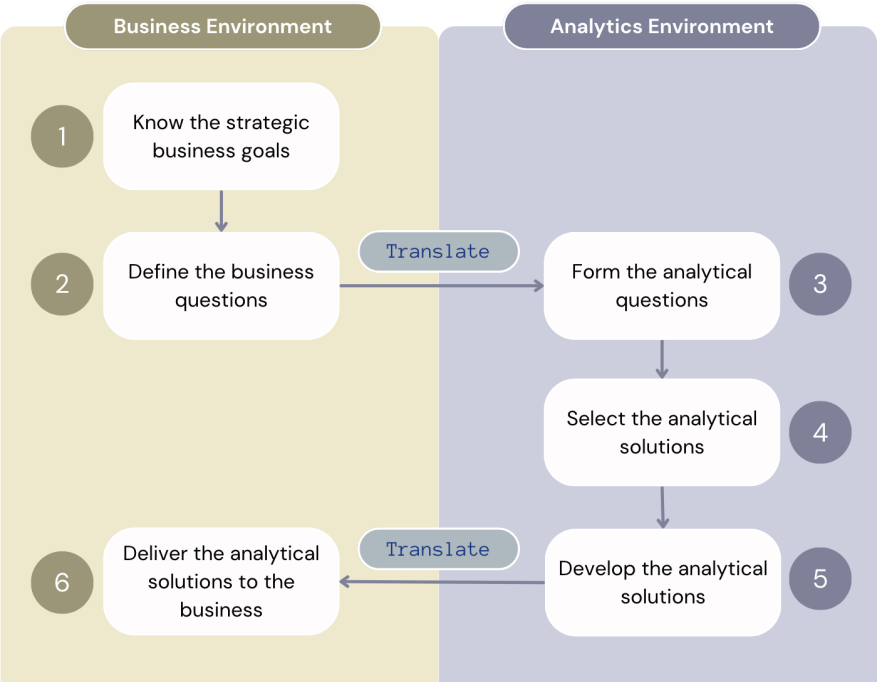
\includegraphics[scale=0.3]{Imagenes/01_Translation.png}
            \label{fig:fig1}
            \end{figure}  
    \end{itemize}
\end{frame}
    % Cuarta diapositiva: Business Questions
    % slide 4
\begin{frame}
    \frametitle{Business Questions}
    \begin{itemize}
        \item<1-> Paso \textbf{1}. Check (grupo directivo)
        \item<1-> Paso \textbf{2}. Check (jefe)
        \item<2-> \underline{Traducir} las \textit{business questions} en \textit{analytical questions} (entre paso \textbf{2} y \textbf{3}).
        \begin{enumerate}
            \item<3-> Entender (palabras clave)
            \item<4-> Identificar (información)
        \end{enumerate}
        \item<5-> Pasos \textbf{4} y \textbf{5}. Creación del \textit{dashboard}
        \item<6-> Paso \textbf{6}. \textit{Data storytelling}
    \end{itemize}
\end{frame}
    % Quinta diapositiva: Palabras Clave
    % slide 5
\begin{frame}
\setbeamercovered{transparent=30}
    \frametitle{Palabras Clave}
    \begin{itemize}
        \item<1-> ¿Cuánto se emitió en la \textbf{CUENTA} \textit{xxx} del \textbf{TRIMESTRE} \textit{ttt}?. En particular enfócate en los \textbf{RAMOS OPERADOS} \textit{aaa}, \textit{bbb} y \textit{ccc}.
        \item<1-> ¿Cuál fue el monto de la cuenta \textit{xxx} por el ramo operado \textit{aaa}?, ¿y el \textbf{AÑO PASADO}?
        \item<1-> ¿Qué empresa es \textbf{LÍDER} en el mercado asegurador en el ramo \textit{aaa}?, ¿dónde \textbf{NOS} encontramos?
        \item<2-> ¿Seguimos la \textbf{TENDENDENCIA} del sector asegurador en la emisión de \textit{aaa}?
        \item<2-> ¿Cómo nos podemos \textbf{COMPARAR} respecto a nuestra competencia?
        \item<3-> ¿Hemos tenido \textbf{CRECIMIENTOS} en los ramos operados \textit{aaa} y \textit{bbb} respecto a ejercicios anteriores?
  \end{itemize}
\end{frame}
    % Sexta diapositiva: Obtener Información
    % slide 6
\begin{frame}
    \frametitle{Obtener información}
    \begin{itemize}
        \item<1-> Información de la empresa
        \item<2-> Información Pública
        \item<3-> Para el caso de seguros recordar lo que nos dice el \textbf{Pilar 3} de \textbf{Solvencia II}
        \item<4->[]
            \begin{figure}[h!]
            \centering
                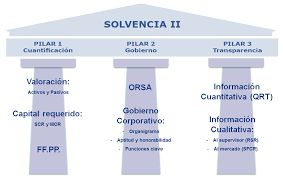
\includegraphics[scale=0.45]{Imagenes/02_Pilares.png}
            \label{fig:fig2}
            \end{figure} 
        \item<5-> \url{https://sio.cnsf.gob.mx/}
  \end{itemize}
\end{frame}
    % Séptima diapositiva: Prepación de base de datos
    % slide 7
\begin{frame}
    \frametitle{Preparación de base de datos}
    \begin{itemize}
        \item<1-> Análisis Exploratorio de los Datos (\textbf{EDA})
        \item<2-> Limpieza
        \item<3-> ¿Se puede \textit{normalizar}?
        \item<4-> Ir a Notebook \codigo{Preparacion.ipynb}
        \item<5-> ¿Por qué crear un \textit{dashboard}?
        \begin{enumerate}
            \item<6-> Interactividad (programación \underline{reactiva})
            \item<7-> Mismas preguntas para valores diferentes
            \item<8-> Tenemos una base de datos ligera
        \end{enumerate}
  \end{itemize}
\end{frame}
    % Octava diapositiva: Programación Reactiva
    % slide 8
\begin{frame}
    \frametitle{Programación Reactiva}
    \begin{itemize}
        \item<1-> \textbf{Reactividad}: cuando los \textit{outputs} reaccionan a los cambios de los \textit{inputs}.
        \item<2-> Cuando una variable \codigo{x} cambia su valor, todo lo relativo a \codigo{x} también cambia su valor. 
        \item<3->  R usa programación reactiva a través de Shiny
        \item<4->[]
        \begin{figure}[h!]
            \centering
                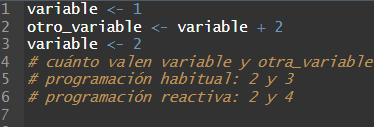
\includegraphics[scale=0.6]{Imagenes/03_Reactividad.png}
            \label{fig:fig3}
            \end{figure} 
  \end{itemize}
\end{frame}
    % Novena diapositiva: Crear un Dashboard en Shiny
    % slide 9
\begin{frame}
    \frametitle{Crear un dashboard en Shiny}
    \begin{itemize}
        \item<1-> En shiny se componen por dos partes:
        \begin{enumerate}
            \item<2-> User Interface (\textbf{UI}): diseño de la interfaz (\textit{frontend})
            \item<3-> Servidor (\textbf{SERVER}): procesamiento de datos (\textit{backend})
        \end{enumerate}
        \item<4-> Primero hay que diseñar la interfaz
        \item<5-> Pues es con la que el usuario va a interactuar
        \item<6-> Para luego tomar los datos del usuario y hacer los procesamientos
        \item<7-> Ir a \url{https://github.com/eruiz1996/Shiny-Notes}
  \end{itemize}
\end{frame}
    % Décima diapositiva: Data-Storytelling
    % slide 10
\begin{frame}
    \frametitle{Data storytelling}
    \begin{itemize}
        \item<1-> En la escuela nos enseñan:
        \begin{enumerate}
            \item<2-> Lengua: estructurar palabras para formar oraciones (\textit{historias})
            \item<3-> Matemáticas: darle sentido a los números (\textit{datos})
        \end{enumerate}
        \item<4-> Nunca nos enseñan a contar historias con datos
        \item<5-> Ser capaz de visualizar y contar historias con los datos es la clave para \textbf{convetir los datos en información} que sirva para la \textbf{toma de decisiones}
        \item<6-> ... \textit{Data is the new oil}
  \end{itemize}
\end{frame}
    % Onceava diapositiva: Diseño del dashboard
    \include{11. Diseño.tex}
    % Doceava diapositiva: Ventajas y desventajas
    % slide 12
\begin{frame}
    \frametitle{Ventajas y desventajas}
    \begin{itemize}
        \item<1-> Ventajas:
        \begin{enumerate}
            \item<2-> Poco código, buen diseño
            \item<3-> Puedes incorporar análisis previos
            \item<4-> Si sabes R (o programar en general) ya llevas más de la mitad
            \item<5-> Incorporar API's (\codigo{Plumber}) e IA
        \end{enumerate}
        \item<6-> Desventajas:
        \begin{enumerate}
            \item<7-> Diseños más específicos necesitan de \codigo{HTML} o \codigo{CSS}
            \item<8-> Si sólo te dedicas hacer dashboards quizá no sea la mejor opción (\textit{Power BI} y \textit{Tableau})
        \end{enumerate}
  \end{itemize}
\end{frame}
    % Doceava diapositiva: Sígueme en mis redes
    \begin{frame}{Sígueme en mis redes sociales}
    \begin{itemize}
        \item[] \faGithub{} GitHub: \url{https://github.com/eruiz1996}
        \item[] \faLinkedin{} LinkedIn: \url{https://www.linkedin.com/in/eruiz1996}
    \end{itemize}
\end{frame}
\end{document}